\documentclass{article}

\usepackage[utf8]{inputenc}
\usepackage[T1]{fontenc}
\usepackage{graphicx}
\usepackage{geometry}
\graphicspath{ {./images/} }
\geometry{a4paper}

\title{Graded Exercise 1}
\author{Duong Le}
\date{}

\begin{document}
\maketitle


\section*{Problem 1}
\subsection*{a.}

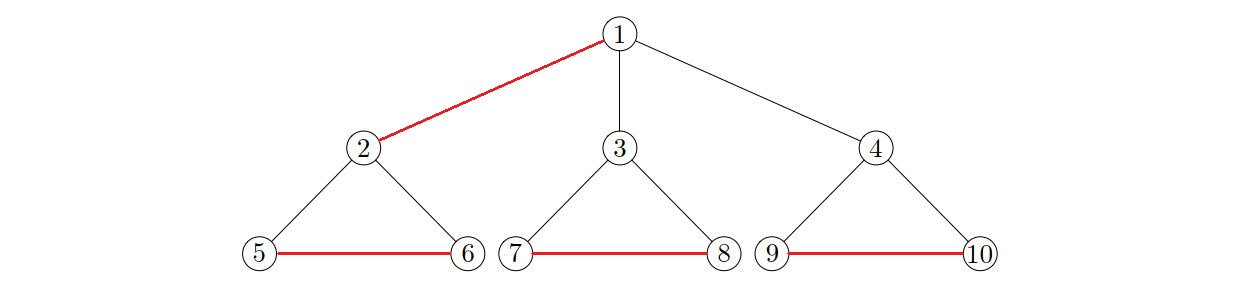
\includegraphics[scale = 0.45]{1a}

The image above illustrates a maximum matching. For each of the three "triangles", a maximum number of one edge can be selected, otherwise it would create an invalid matching. And for the three edges branching from vertex (1), only one edge can be matched. So the maximum number of edges in a match is:

\[ n = 1 + 3 = 4 \]

So the matching presented is a maximum matching.
\pagebreak

\subsection*{b.}

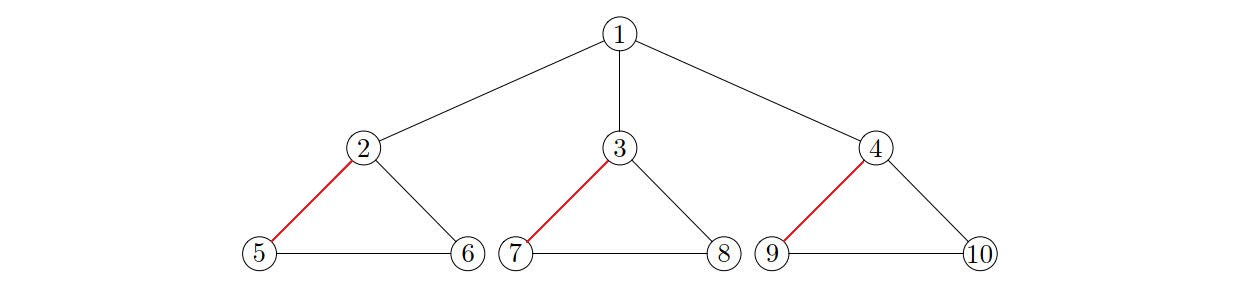
\includegraphics[scale = 0.45]{1b}

The image above illustrates a maximal matching. Without loss of generality, consider the subgraph consists of the edges (2), (5), and (6):

\begin{itemize}
    \item If we include the edges \{ (2), (6) \}, vertex (2) will be invalid.
    \item If we include the edges \{ (5), (6) \}, vertex (6) will be invalid.
    \item If we include the edges \{ (1), (2) \}, vertex (2) will be invalid.
\end{itemize}	

So the matching presented is a maximal matching.
\pagebreak


\section*{Problem 2}
Consider the cycle (1) $\rightarrow$ (5) $\rightarrow$ (4) $\rightarrow$ (3) $\rightarrow$ (2) $\rightarrow$ (1). The cycle has an odd number of vertices \\
$\Rightarrow$ The chromatic number of the graph is at least 3. \\\\
Assume that the chromatic number of the graph is 3, and denote the colors as "a", "b", and "c". \\
Without loss of generality, let the vertex (1) has the color "a". We then have two cases, either the vertices (5) and (2) have the same colors, or they have different colors. \\

\subsection*{2.1. (2) and (5) have different colors}
\begin{itemize}
    \item Since (2) and (5) have different colors, (6) must have color "a". This means (11) cannot have color "a". We also assume that, wlog, (5) has color "b" and (2) has color "c".
    \item At this point, there are two cases for the vertices (4) and (3): They can assume the colors "c" and "b" respectively, or one of them can have the color "a".
    \begin{itemize}
         \item Assume that (4) has color "a" and (3) has color "b". Then the colors of (8) and (7) must be "b" and "c" respectively. That means (11)'s color must be            "a". We have a contradiction since the color of (11) cannot be "a" (See the left picture of Figure 1).
         \item We can argue the same if (4) has color "c" and (3) has color "a".
         \item If (4) has color "c" and (3) has color "b". Then (10) and (7) must have colors "b" and "c" respectively. That means (11)'s color must be "a". We arrive at the same contradiction (See the right picture of Figure 1).
     \end{itemize}               
\end{itemize}
$\Rightarrow$ If colored in this way, at least 4 colors is needed.

\begin{figure}[h]
    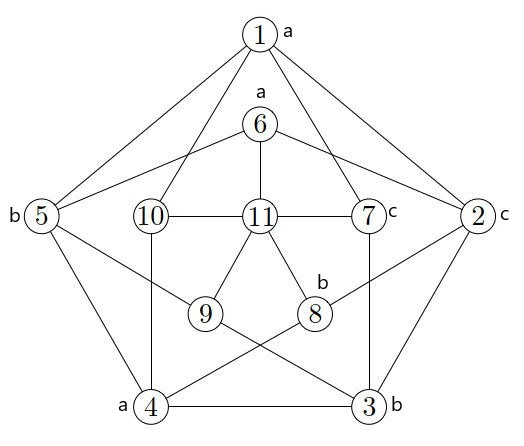
\includegraphics[scale = 0.53]{2.1.a}
    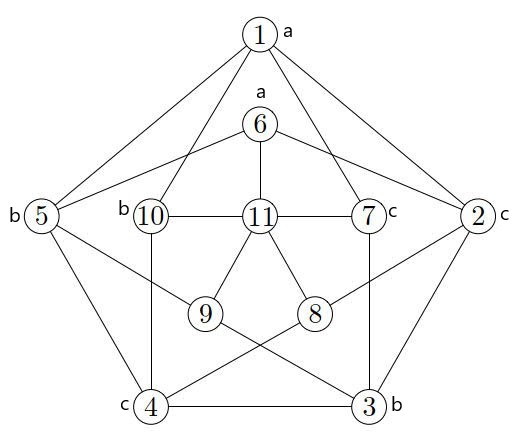
\includegraphics[scale = 0.53]{2.1.b}
    \caption{The graph if (5) and (2) have different colors.}
\end{figure}

\subsection*{2.2. (2) and (5) have same colors}
\begin{itemize}
    \item Assume, without loss of generality, (5) and (2) have color "b". Then (4) and (3) can only take the colors "a" and "c".
    \item Let (4) has the color "a" and (3) has the color "c". Then we can conclude the following:
    \begin{itemize}
        \item The color of (7) can only be "b". So (11) cannot take the color "b".
        \item The color of (8) can only be "c". So (11) cannot take the color "c".
        \item The color of (9) can only be "a". So (11) cannot take the color "a".
    \end{itemize}
\end{itemize}
$\Rightarrow$ If colored in this way, at least 4 colors is needed. We can argue similarly if (4) takes the color "c" and (3) takes "a".

\begin{figure}[h]
    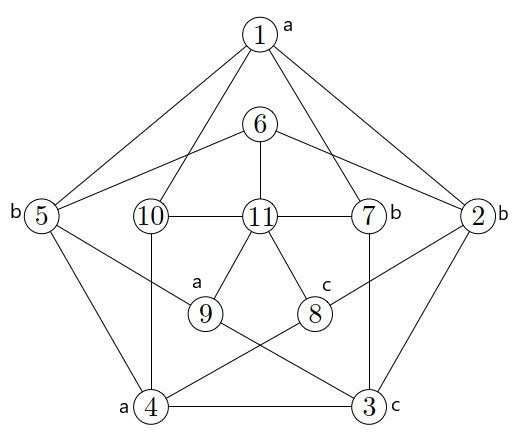
\includegraphics[scale = 0.53]{2.2}
    \centering
    \caption{The graph if (5) and (2) have same colors.}
\end{figure}

$\Longrightarrow$ From 2.1 and 2.2, we can conclude that the graph cannot be colored using 3 colors. \\\\
Below is an example of the graph colored using 4 colors "a", "b", "c", and "d".

\begin{figure}[h]
    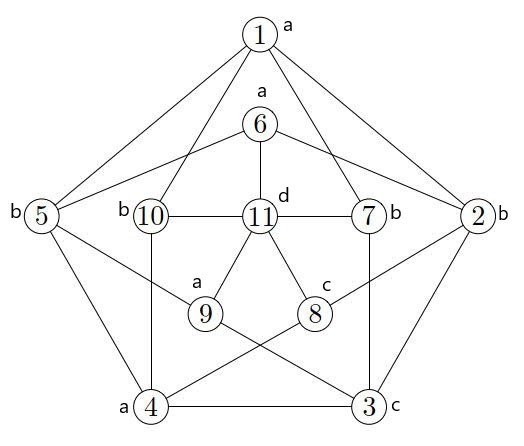
\includegraphics[scale = 0.53]{2.3}
    \centering
    \caption{The graph coloring using 4 colors.}
\end{figure}

$\Longrightarrow$ The chromatic number of the graph is 4.
\pagebreak


\section*{Problem 3}
The problem asks to prove that in trees, each node of degree 3 or more can be mapped to at least on unique leaf node. To prove this, we can show that in a tree, the number of node with degree 3 or more is always less than the number of leaf nodes (nodes with degree 1).  \\\\
Let the degree of a node and the set of all possible degrees in the tree denoted as ${d}$ and ${D}$ respectively. Also denote the number of nodes with degree ${d}$ as ${v_d}$. We have, using the handshaking lemma: 

\[ \sum_{d \in D} {v_d}  {d} = 2|{E}|\] 

We also know that, the number of edges in a tree is equal to the number of nodes minus 1. So the above sum can be written as:

\[ \sum_{d \in D} {v_d}  {d} = 2(\sum_{d \in D} {v_d} - 1)\]
$\Leftrightarrow$ 
\[\sum_{d \in D} {v_d}  {d} = \sum_{d \in D} {2v_d} - 2\]
$\Leftrightarrow$ 
\[ 2 = \sum_{d \in D} {2v_d} - \sum_{d \in D} {v_d}  {d} = \sum_{d \in D} {(2 - d)v_d}\]

Since 2 > 0, the left hand side must be positive. Consider, the term ${(2 - d)v_d}$ would be 0 if ${d = 2}$ and negative if ${d \geq 3}$. \\\\
$\Rightarrow$ In order for the right hand side to be positive, ${v_d}$ when ${d = 1}$ must be larger than the sum of ${v_d}$ when ${d \geq 3}$. In other words, the number of nodes with degree 1 must be greater than the number of nodes with degree 3 or more.







\end{document}